\documentclass[tikz, border=15pt]{standalone}
\usepackage[T1]{fontenc}
\usepackage{helvet}
\renewcommand{\familydefault}{\sfdefault}
\usetikzlibrary{positioning, calc, arrows.meta}

\definecolor{attncolor}{HTML}{FCE8E6}       % Soft Red/Coral (Multi-Head Attention)
\definecolor{maskedattncolor}{HTML}{FEF7E0} % Soft Yellow (Masked Multi-Head Attention)
\definecolor{ffcolor}{HTML}{E8F0FE}         % Soft Blue (Feed Forward)
\definecolor{normcolor}{HTML}{E6F4EA}       % Soft Green (Add & Norm)
\definecolor{embcolor}{HTML}{F1F3F4}        % Soft Light Gray (Embeddings)
\definecolor{lincolor}{HTML}{F3E8FD}        % Soft Purple (Linear/Softmax)
\definecolor{pecolor}{HTML}{ECEFF1}         % Soft Slate Gray (Positional Encoding)

\begin{document}
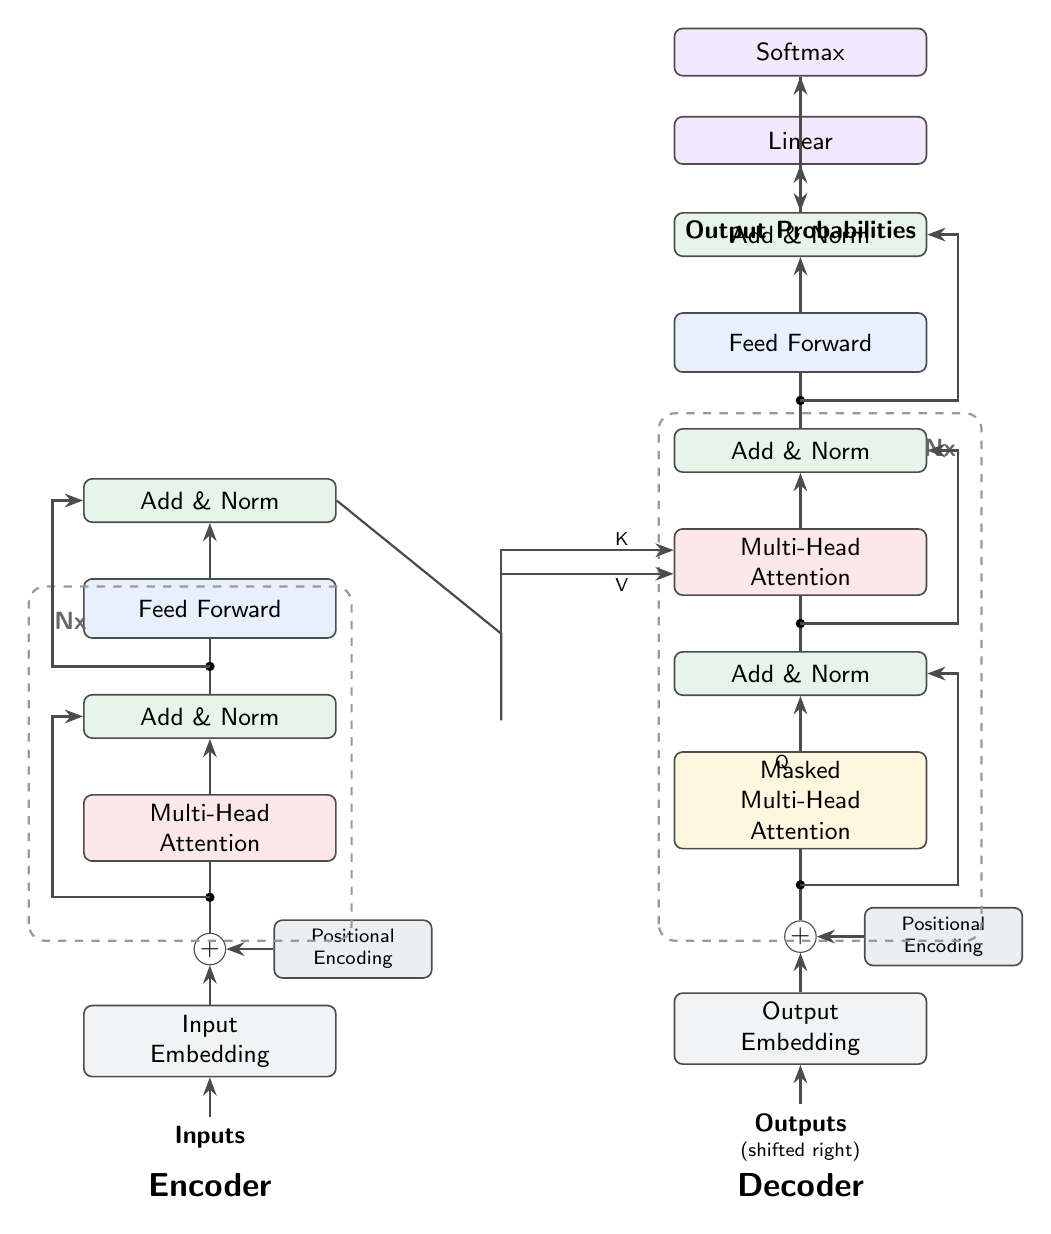
\begin{tikzpicture}[
    node distance=1cm and 1.5cm,
    align=center,
    font=\sffamily\small,
    block/.style={draw=black!70, rectangle, minimum width=3.2cm, minimum height=0.75cm, rounded corners=3pt, line width=0.6pt, align=center},
    attn/.style={block, fill=attncolor},
    maskedattn/.style={block, fill=maskedattncolor},
    ff/.style={block, fill=ffcolor},
    norm/.style={block, fill=normcolor, minimum height=0.55cm},
    emb/.style={block, fill=embcolor},
    lin/.style={block, fill=lincolor, minimum height=0.6cm},
    pe/.style={block, fill=pecolor, minimum width=2.0cm, minimum height=0.6cm, font=\sffamily\scriptsize},
    arrow/.style={-Stealth, thick, draw=black!70},
    line/.style={thick, draw=black!70}
]

    % =========================================================================
    % ENCODER STACK
    % =========================================================================
    
    % Input layers
    \node (in_lbl) at (0, 0) {\textbf{Inputs}};
    \node (in_emb) [emb, above=0.5cm of in_lbl] {Input\\Embedding};
    \node (in_pe_plus) [draw=black!70, circle, minimum size=0.4cm, inner sep=0pt, above=0.5cm of in_emb] {+};
    \node (in_pe) [pe, right=0.6cm of in_pe_plus] {Positional\\Encoding};
    
    % Stack layers
    \node (enc_attn) [attn, above=0.9cm of in_pe_plus] {Multi-Head\\Attention};
    \node (enc_norm1) [norm, above=0.7cm of enc_attn] {Add \& Norm};
    \node (enc_ff) [ff, above=0.7cm of enc_norm1] {Feed Forward};
    \node (enc_norm2) [norm, above=0.7cm of enc_ff] {Add \& Norm};
    
    % Encoder Stack Box (Nx)
    \draw [draw=black!40, dashed, rounded corners=6pt, line width=0.8pt] (-2.3, 2.5) rectangle (1.8, 7.0);
    \node at (-2.1, 6.8) [anchor=north west, font=\sffamily\bfseries\small, text=black!60] {Nx};

    % Connections & Residuals
    \draw [arrow] (in_lbl) -- (in_emb);
    \draw [arrow] (in_emb) -- (in_pe_plus);
    \draw [arrow] (in_pe) -- (in_pe_plus);
    
    \draw [line] (in_pe_plus) -- (enc_attn) node[midway, circle, fill=black, inner sep=1.2pt] (enc_res1_pt) {};
    \draw [arrow] (enc_res1_pt.center) -- ++(-2.0, 0) |- (enc_norm1.west);
    \draw [arrow] (enc_attn) -- (enc_norm1);
    
    \draw [line] (enc_norm1) -- (enc_ff) node[midway, circle, fill=black, inner sep=1.2pt] (enc_res2_pt) {};
    \draw [arrow] (enc_res2_pt.center) -- ++(-2.0, 0) |- (enc_norm2.west);
    \draw [arrow] (enc_ff) -- (enc_norm2);
    
    % Label
    \node at (0, -0.6) [font=\sffamily\bfseries\large] {Encoder};


    % =========================================================================
    % DECODER STACK
    % =========================================================================
    
    % Output layers
    \node (out_lbl) at (7.5, 0) {\textbf{Outputs}\\[-2pt]\scriptsize(shifted right)};
    \node (out_emb) [emb, above=0.5cm of out_lbl] {Output\\Embedding};
    \node (out_pe_plus) [draw=black!70, circle, minimum size=0.4cm, inner sep=0pt, above=0.5cm of out_emb] {+};
    \node (out_pe) [pe, right=0.6cm of out_pe_plus] {Positional\\Encoding};
    
    % Stack layers
    \node (dec_masked_attn) [maskedattn, above=0.9cm of out_pe_plus] {Masked\\Multi-Head\\Attention};
    \node (dec_norm1) [norm, above=0.7cm of dec_masked_attn] {Add \& Norm};
    \node (dec_cross_attn) [attn, above=0.7cm of dec_norm1] {Multi-Head\\Attention};
    \node (dec_norm2) [norm, above=0.7cm of dec_cross_attn] {Add \& Norm};
    \node (dec_ff) [ff, above=0.7cm of dec_norm2] {Feed Forward};
    \node (dec_norm3) [norm, above=0.7cm of dec_ff] {Add \& Norm};
    
    % Output prediction layers
    \node (dec_linear) [lin, above=0.6cm of dec_norm3] {Linear};
    \node (dec_softmax) [lin, above=0.5cm of dec_linear] {Softmax};
    \node (out_probs) at (7.5, 11.5) {\textbf{Output Probabilities}};
    
    % Decoder Stack Box (Nx)
    \draw [draw=black!40, dashed, rounded corners=6pt, line width=0.8pt] (5.7, 2.5) rectangle (9.8, 9.2);
    \node at (9.6, 9.0) [anchor=north east, font=\sffamily\bfseries\small, text=black!60] {Nx};

    % Connections & Residuals
    \draw [arrow] (out_lbl) -- (out_emb);
    \draw [arrow] (out_emb) -- (out_pe_plus);
    \draw [arrow] (out_pe) -- (out_pe_plus);
    
    \draw [line] (out_pe_plus) -- (dec_masked_attn) node[midway, circle, fill=black, inner sep=1.2pt] (dec_res1_pt) {};
    \draw [arrow] (dec_res1_pt.center) -- ++(2.0, 0) |- (dec_norm1.east);
    \draw [arrow] (dec_masked_attn) -- (dec_norm1);
    
    \draw [line] (dec_norm1) -- (dec_cross_attn) node[midway, circle, fill=black, inner sep=1.2pt] (dec_res2_pt) {};
    \draw [arrow] (dec_res2_pt.center) -- ++(2.0, 0) |- (dec_norm2.east);
    \draw [arrow] (dec_cross_attn) -- (dec_norm2);
    
    \draw [line] (dec_norm2) -- (dec_ff) node[midway, circle, fill=black, inner sep=1.2pt] (dec_res3_pt) {};
    \draw [arrow] (dec_res3_pt.center) -- ++(2.0, 0) |- (dec_norm3.east);
    \draw [arrow] (dec_ff) -- (dec_norm3);
    
    \draw [arrow] (dec_norm3) -- (dec_linear);
    \draw [arrow] (dec_linear) -- (dec_softmax);
    \draw [arrow] (dec_softmax) -- (out_probs);
    
    % Label
    \node at (7.5, -0.6) [font=\sffamily\bfseries\large] {Decoder};


    % =========================================================================
    % CROSS-ATTENTION CONNECTIONS (ENCODER -> DECODER)
    % =========================================================================
    \coordinate (split_pt) at (3.7, 5.3);
    \draw [line] (enc_norm2.east) -- (3.7, 6.4) -- (split_pt);
    \draw [arrow] (split_pt) |- ($(dec_cross_attn.west) + (0, 0.15)$) node[pos=0.85, above=-1pt, scale=0.75] {K};
    \draw [arrow] (split_pt) |- ($(dec_cross_attn.west) + (0, -0.15)$) node[pos=0.85, below=-1pt, scale=0.75] {V};
    
    % Q connection label
    \node at (7.5, 4.75) [left, scale=0.75, xshift=-2pt] {Q};

\end{tikzpicture}
\end{document}
